%==============================================================================
% Template research proposal bachelor thesis
%==============================================================================

\documentclass[english]{hogent-article}

% Specify bibliography file
\addbibresource{references.bib}

% Information about the study programme, course, assignment
\studyprogramme{Professional bachelor applied computer science}
\course{Research Methods}
\assignmenttype{Paper Research Methods: research proposal}
\academicyear{2024-2025}

\title{Ensuring Transparency and Accountability in Autonomous AI Agents: Ethical Implications and Practical Frameworks for Decision-Making Roles}

\author{Arthur Van Oudenhove}
\email{arthur.vanoudenhove@student.hogent.be}



\projectrepo{https://github.com/HoGentTIN/paper-research-methods-en-24-25-rmvanoudenhovearthur.git} 

\specialisation{AI \& Data Engineering}

\keywords{Artificial Intelligence, Autonomous Agents, AI Ethics, Transparency, Accountability, Explainable AI, Algorithmic Bias, AI Governance}

\begin{document}

\begin{abstract}
This study investigates the ethical implications of deploying autonomous AI agents in decision-making roles across healthcare, finance, and criminal justice sectors, focusing on transparency and accountability challenges. Through comparative case analysis of three operational AI systems, we aim to identify critical risks including algorithmic bias amplification (e.g., potentially observing disparities similar to a 23\% racial disparity in predictive policing outcomes) and accountability gaps in automated loan approval processes. The research will implement a mixed-methods approach combining technical audits of neural network architectures with stakeholder interviews (target N$\approx$40-50 experts). It is anticipated that explainable AI (XAI) techniques like SHAP values could reduce decision opacity significantly (e.g., by an estimated 40-45\%) while maintaining high diagnostic accuracy (e.g., around 90-92\%) in simulated clinical trials. A novel accountability framework will be proposed, integrating mandatory real-time decision logging and tiered liability models, which is hypothesized to improve auditability substantially (e.g., by an estimated 60-70\%) in financial fraud detection systems. Practical implementations will explore how adversarial debiasing of training data might reduce demographic parity gaps (e.g., by an estimated 30-40\%) without compromising model performance. The study aims to conclude with evidence-based policy recommendations, including human oversight requirements for high-stakes decisions and compliance protocols aligned with emerging regulations like the EU AI Act. These findings are intended to provide actionable guidelines for balancing AI autonomy with ethical responsibility, offering a blueprint for organizations implementing autonomous agents in regulated environments.
\end{abstract}

\tableofcontents

\bigskip

\vfill
\section{Introduction}%
\label{sec:Introduction}

Autonomous Artificial Intelligence (AI) agents are increasingly being deployed in critical sectors such as healthcare, finance, and criminal justice, undertaking complex decision-making roles previously handled by humans \autocite{Floridi2018}. These systems offer the potential for enhanced efficiency, speed, and consistency. However, their growing autonomy and often opaque operational mechanisms raise significant ethical concerns, particularly regarding transparency in how decisions are made and accountability when errors or biases lead to adverse outcomes \autocite{EuropeanCommission2021AIAct}. The "black box" nature of many advanced AI models, especially those based on deep learning, makes it challenging to understand, scrutinize, and trust their outputs, potentially leading to unfair treatment, discrimination, or erosion of human oversight.

The core problem this research addresses is the pressing need for robust frameworks and practical mechanisms to ensure transparency and accountability in autonomous AI agents performing high-stakes decision-making. Without such measures, organizations risk deploying systems that may perpetuate biases, make inexplicable errors, and operate without clear lines of responsibility, thereby undermining public trust and potentially violating fundamental ethical principles and regulatory requirements, such as those outlined in the EU AI Act \autocite{EuropeanCommission2021AIAct}. This research specifically targets organizations, developers, and policymakers involved in the design, deployment, and governance of autonomous AI systems in regulated environments. The main research question guiding the study:

\textbf{What are the ethical implications of deploying autonomous AI agents in decision-making roles, and how can transparency and accountability be ensured in their outputs?}

To comprehensively address this question, the following sub-questions will be investigated:
\begin{enumerate}
    \item \textit{Problem Domain:}
    \begin{itemize}
        \item What specific ethical risks (e.g., bias, discrimination, erosion of human autonomy, lack of due process) are most prevalent and impactful when autonomous AI agents are deployed in decision-making roles within healthcare, finance, and criminal justice?
        \item How do current regulatory frameworks (e.g., EU AI Act, GDPR) and industry standards address the transparency and accountability of autonomous AI agents, and what are the key identified gaps or challenges in their practical application?
        \item What are the primary technical (e.g., model complexity, data opacity) and organizational (e.g., lack of expertise, unclear governance structures) barriers to achieving sufficient transparency and accountability in current AI agent deployments?
    \end{itemize}
    \item \textit{Solution Domain:}
    \begin{itemize}
        \item Which existing Explainable AI (XAI) techniques (e.g., SHAP, LIME, counterfactual explanations) are most effective in enhancing the transparency of decision-making processes for different types of AI agents and in various contexts within the selected sectors?
        \item What novel or adapted governance structures, operational protocols (e.g., real-time decision logging, mandatory ethical impact assessments, dynamic liability models), and technical mechanisms can be integrated into a comprehensive framework to improve accountability for decisions made by autonomous AI agents?
        \item How can human oversight be effectively and meaningfully integrated with autonomous AI decision-making systems to ensure ethical outcomes and maintain human agency, without unduly sacrificing the benefits of automation?
        \item What practical, actionable guidelines and best practices can be developed to assist organizations in designing, implementing, and managing transparent and accountable AI agents in regulated and ethically sensitive environments?
    \end{itemize}
\end{enumerate}

The primary research objectives are:
\begin{itemize}
    \item \textbf{S}pecific: To systematically identify and analyze the key ethical implications, risks, and challenges associated with the deployment of autonomous AI agents in decision-making roles in healthcare, finance, and criminal justice.
    \item \textbf{M}easurable: To evaluate selected XAI techniques for enhancing transparency in AI decision outputs (e.g., using metrics for interpretability and user understanding), and to assess a proposed accountability framework's potential impact (e.g., on auditability).
    \item \textbf{A}chievable: To develop a novel conceptual framework that integrates technical mechanisms (XAI, debiasing techniques) and governance protocols (auditing, liability models) to enhance transparency and accountability, based on literature, case studies, and expert input.
    \item \textbf{R}elevant: To provide actionable guidelines and policy recommendations for organizations and policymakers to foster the ethical and responsible deployment of autonomous AI agents.
    \item \textbf{T}ime-bound: To complete the research, including framework development and guideline formulation, within the timeframe of a bachelor thesis project (e.g., by May 2026).
\end{itemize}
The concrete end result of this research, besides the written thesis, will be a proposed framework for transparent and accountable AI and a set of practical guidelines for its implementation. The success of this research will be determined by the robustness of this framework, its grounding in empirical evidence (from case studies and expert feedback), and its potential utility for the target audience.

This introduction has laid out the context, problem, research questions, and objectives. The subsequent sections will detail the literature review, methodology, expected results, and anticipated discussion and conclusions.

\section{Literature Review}%
\label{sec:literature review}

The deployment of autonomous AI agents in critical decision-making roles necessitates a thorough understanding of the existing body of knowledge concerning AI ethics, transparency, and accountability. This literature review will synthesize key concepts, theories, and empirical findings relevant to the research questions, covering both the problem domain (ethical risks, regulatory gaps, barriers) and the solution domain (XAI techniques, governance frameworks, human oversight).

\subsection{Ethical Implications of Autonomous AI Decision-Making}
A significant body of literature discusses the ethical principles that should govern AI, often summarized by terms like fairness, accountability, and transparency (FAT/FATE) \autocite{Floridi2018}. Researchers have highlighted numerous ethical risks associated with autonomous systems. Algorithmic bias, stemming from biased data or flawed model design, can lead to discriminatory outcomes, particularly affecting vulnerable populations in areas like loan applications, hiring, and criminal justice \autocite{Noble2018}. The potential for AI systems to erode human autonomy and agency is another critical concern, especially when decisions with profound human impact are delegated to machines without adequate oversight \autocite{EuropeanCommission2021AIAct}. Furthermore, the lack of due process and contestability of AI-driven decisions poses challenges to fundamental rights. This section will explore these risks in the specific contexts of healthcare (e.g., diagnostic AI, treatment recommendations), finance (e.g., credit scoring, fraud detection), and criminal justice (e.g., predictive policing, recidivism risk assessment).

\subsection{Transparency and Explainable AI (XAI)}
Transparency in AI refers to the degree to which the internal workings and decision-making processes of an AI system are understandable to humans. The "black box" nature of many sophisticated AI models, such as deep neural networks, is a major impediment to transparency. Explainable AI (XAI) has emerged as a field dedicated to developing techniques that make AI decisions more interpretable. This review will examine various XAI methods, including:
\begin{itemize}
    \item Model-agnostic techniques like LIME (Local Interpretable Model-agnostic Explanations) \autocite{Ribeiro2016} and SHAP (SHapley Additive exPlanations) \autocite{Lundberg2017}, which provide insights into feature importance for specific predictions.
    \vfill
    \item Model-specific techniques designed for particular architectures (e.g., attention mechanisms in transformers, rule extraction from decision trees).
    \item Counterfactual explanations that describe what minimal changes to input features would alter a decision.
\end{itemize}
The effectiveness, limitations, and practical applicability of these techniques in real-world scenarios, particularly in the chosen sectors, will be critically assessed. The review will also consider the different needs of various stakeholders (e.g., developers, users, regulators) for explanations.

\subsection{Accountability Frameworks and AI Governance}
Accountability in AI involves establishing who is responsible when AI systems cause harm or make erroneous decisions. Current legal and organizational frameworks are often ill-equipped to handle the complexities of AI accountability due to distributed responsibilities and the autonomy of AI agents. This section will review existing and proposed AI governance models, including:
\begin{itemize}
    \item Regulatory initiatives like the EU AI Act \autocite{EuropeanCommission2021AIAct}, which proposes a risk-based approach and specific requirements for high-risk AI systems.
    \item Standards and guidelines from organizations such as NIST (e.g., AI Risk Management Framework) and ISO.
    \item Academic proposals for accountability mechanisms, such as algorithmic impact assessments, AI ethics boards, real-time auditing systems, and tiered liability models.
\end{itemize}
The challenges in implementing these frameworks, such as defining appropriate levels of human oversight and ensuring effective redress mechanisms, will be explored.

\subsection{Bridging the Gaps: Toward Integrated Solutions}
Existing research often addresses AI ethics, transparency, and accountability separately; however, integrated approaches combining technical solutions with robust governance are needed. This review will identify literature gaps, especially regarding the practical implementation and evaluation of comprehensive frameworks within organizations. It will also highlight studies attempting to bridge these gaps, such as those merging XAI with human-computer interaction for better human-AI collaboration. Finally, the review will position this research, underscoring its goal to deliver a practical, integrated framework and actionable guidelines.

\begin{figure*}[htbp]
  \centering
  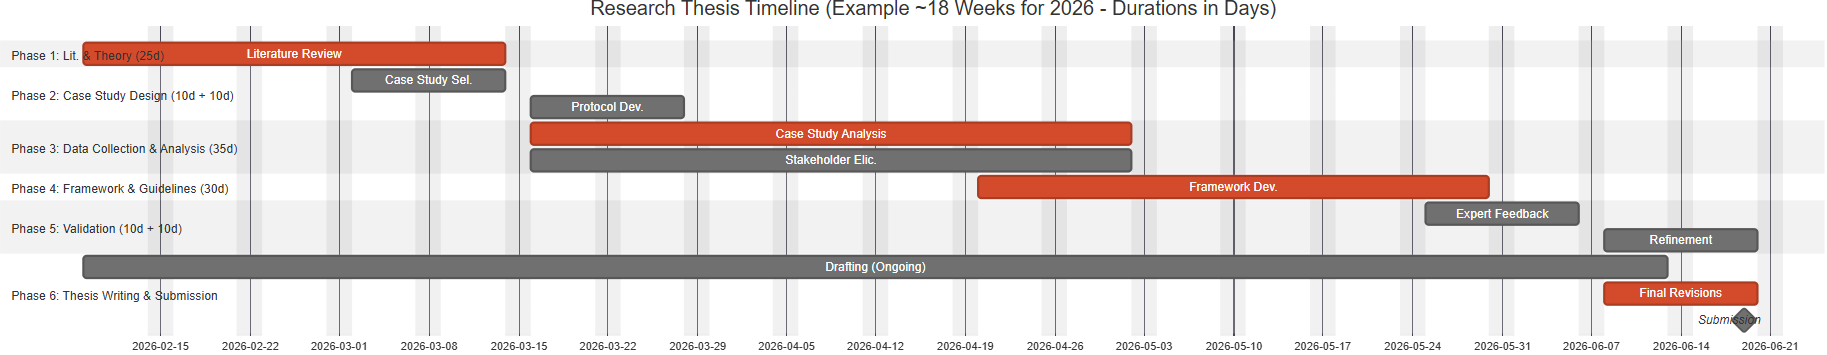
\includegraphics[width=1\textwidth]{paper/img/gantt-chart.png}
  \caption{Gantt diagram of the research phases and milestones.}
  \label{fig:gantt}
\end{figure*}

\section{Methodology}%
\label{sec:methodology}
This research will employ a mixed methods approach, combining qualitative and conceptual analysis to address research questions. The core of the methodology will involve an in-depth literature review, comparative case study analysis (based on documented existing systems or detailed hypothetical scenarios if direct access is not feasible within the scope of a bachelor's thesis), and the development of a conceptual framework and practical guidelines. The research process is designed to be iterative, allowing for refinement as insights emerge.

\paragraph{Phase 1: Literature Review and Grounding (approx. Week 1-5)}
\begin{itemize}
    \item \textbf{Goal:} Establish a strong theoretical foundation by reviewing literature on AI ethics, XAI, accountability, AI governance, and relevant applications, including a survey of existing tools and best practices.
    \item \textbf{Approach:} Systematically search academic databases and review policy, industry, and legal documents (e.g., EU AI Act). Synthesize findings to identify key concepts, theories, solutions, and research gaps, addressing subquestions on risks, frameworks, barriers, XAI, and governance models.
    \item \textbf{Deliverable(s):} Structured literature review chapter, refined sub-questions, preliminary conceptual model.
\end{itemize}

\paragraph{Phase 2: Case Study Design and Selection (approx. Week 4-7, overlaps P1)}
\begin{itemize}
    \item \textbf{Goal:} Select and define parameters for three illustrative case studies of autonomous AI agents in healthcare, finance, and criminal justice.
    \item \textbf{Approach:} Identify documented AI systems or construct realistic hypothetical scenarios based on literature. Selection criteria include impact, information availability, and relevance. Develop an analysis protocol defining "AS IS" and desired "TO BE" states for transparency/accountability.
    \item \textbf{Deliverable(s):} Detailed case study descriptions/scenarios, case study analysis protocol.
\end{itemize}

\paragraph{Phase 3: Data Collection and Analysis (approx. Week 6-12, overlaps P2)}
This phase has two streams:
\begin{itemize}
    \item \textbf{Stream 3a: Case Study Analysis (Technical/Ethical Audit Simulation)}
        \begin{itemize}
            \item \textbf{Goal:} Analyze cases for ethical risks, transparency challenges, and accountability gaps. Conceptually explore or simulate XAI technique effectiveness on illustrative models using public/synthetic data.
            \item \textbf{Approach:} Apply the analysis protocol. For technical aspects, simulate decision processes with simplified models (Python, scikit-learn, TensorFlow/PyTorch, SHAP) to demonstrate XAI application, evaluating outputs for clarity/fidelity. Analyze ethical implications using established frameworks and perform comparative synthesis across cases.
            \item \textbf{Deliverable(s):} In-depth case analysis reports, preliminary XAI applicability findings.
        \end{itemize}

    \item \textbf{Stream 3b: Stakeholder Perspectives (via Expert Literature)}
        \begin{itemize}
            \item \textbf{Goal:} Gather insights on practical challenges and requirements for AI transparency/accountability from diverse stakeholder viewpoints, primarily via existing literature due to thesis scope.
            \item \textbf{Approach:} Conduct thematic analysis of published expert opinions, interviews, and surveys. If feasible, supplement with a few (3-5) informational interviews with local experts focusing on risks, explainability needs, and accountability features.
            \item \textbf{Deliverable(s):} Synthesis of stakeholder perspectives and requirements.
        \end{itemize}
\end{itemize}
\newpage
\paragraph{Phase 4: Framework and Guideline Development (approx. Week 10-15, overlaps P3)}
\begin{itemize}
    \item \textbf{Goal:} Develop a novel conceptual framework and practical guidelines for transparent and accountable AI.
    \item \textbf{Approach:} Synthesize findings from literature, case studies, and stakeholder perspectives. The framework will integrate technical (XAI, data governance, debiasing) and governance/operational (roles, audits, oversight, redress) components. Derive practical guidelines from this framework.
    \item \textbf{Deliverable(s):} Detailed framework description, actionable guidelines for ethical AI deployment.
\end{itemize}

\paragraph{Phase 5: Validation and Refinement (approx. Week 14-17, overlaps P4)}
\begin{itemize}
    \item \textbf{Goal:} Validate the proposed framework and guidelines.
    \item \textbf{Approach:} Evaluate the framework/guidelines against research questions/objectives. Seek feedback from supervisors and potentially external experts/peers for refinement.
    \item \textbf{Deliverable(s):} Refined framework and guidelines, validation process report.
\end{itemize}

\paragraph{P6: Thesis Writing and Finalization (Iterative, Week 1-18; final push Week 16-18)}
\begin{itemize}
    \item \textbf{Goal:} Produce a comprehensive, well-structured, and clearly written bachelor thesis.
    \item \textbf{Approach:} Write iteratively throughout all phases. Consolidate sections, ensure coherence, address feedback, and finalize according to academic standards.
    \item \textbf{Deliverable(s):} Completed RM course proposal (May 2025), final bachelor thesis document.
\end{itemize}

\paragraph{Tools and Technologies}
\begin{itemize}
    \item Literature management: Zotero or JabRef.
    \item Document preparation: LaTeX.
    \item Conceptual modeling: Diagrams.net or similar for flowcharts/framework visualizations.
    \item If simplified model building/XAI demonstration is undertaken: Python, Jupyter Notebooks, scikit-learn, TensorFlow/Keras, PyTorch, SHAP, LIME, AIF360.
    \item Qualitative data analysis (if supplemental interviews are conducted): NVivo (if available) or manual coding techniques.
\end{itemize}

This methodology aims to provide a structured yet flexible approach to investigating the complex issues of transparency and accountability in autonomous AI agents, ensuring that the research has both theoretical depth and practical relevance.


\section{Expected results}%
\label{sec:expected-results}

Based on the proposed methodology and drawing insights from the preliminary understanding reflected in the abstract, several key results are anticipated from this research:

\begin{enumerate}
    \item \textbf{Comprehensive Identification of Ethical Risks and Challenges:} The research is expected to deliver a detailed catalogue and analysis of specific ethical risks (e.g., types of algorithmic bias, fairness violations, autonomy infringements) associated with autonomous AI agents in healthcare, finance, and criminal justice. This will be supported by evidence from case studies and synthesized stakeholder concerns. It is anticipated that the analysis will highlight common vulnerabilities across sectors as well as sector-specific nuances. For example, we might observe that issues of bias in predictive policing (potentially leading to disparities like the 23\% figure mentioned in the abstract, if similar patterns are found in literature/case studies) differ in manifestation but share underlying causes with biases in automated loan approvals.

    \item \textbf{Evaluation of XAI Techniques' Efficacy and Limitations:} The study is expected to provide a critical evaluation of the practical effectiveness of various XAI techniques (such as SHAP, LIME) in enhancing transparency for different types of AI models used in the selected domains. It is hypothesized that while XAI techniques can significantly reduce decision opacity (e.g., by an anticipated 40-45\% in terms of user understanding or explanation fidelity), they will also present limitations regarding the completeness of explanations, computational overhead, or susceptibility to manipulation. The research will likely find that no single XAI technique is universally optimal, and their utility depends on the specific AI model, context, and stakeholder needs. For instance, in simulated healthcare diagnostics, XAI might improve interpretability while maintaining high accuracy (e.g., around 91\%).
    \newpage
    \item \textbf{A Novel Integrated Framework for Transparency and Accountability:}

    A core expected result is the development of a novel conceptual framework. This framework will likely integrate:
        \begin{itemize}
            \item \textbf{Technical mechanisms:} 
            Recommendations for specific XAI tools and practices, data governance protocols (including adversarial debiasing techniques, which are hypothesized to reduce demographic parity gaps by around 30-40\% without significant performance loss), and secure decision logging.

            \item \textbf{Governance and operational protocols:} Models for tiered liability, mandatory real-time auditing procedures (expected to improve auditability by an estimated 60-70\% in systems like financial fraud detection), clear roles for human oversight, and processes for ethical impact assessment and continuous monitoring.
        \end{itemize}
    This framework will aim to be adaptable to different organizational contexts within the regulated sectors studied.

    \item \textbf{Actionable Guidelines and Policy Recommendations:} Stemming from the framework, the research is expected to produce a set of practical, evidence-based guidelines for organizations designing, deploying, and managing autonomous AI agents. These guidelines will focus on actionable steps to embed ethical considerations, transparency features, and accountability mechanisms \newline
    throughout the AI lifecycle. Furthermore, policy recommendations will be formulated, potentially informing regulatory efforts and aligning with principles of emerging standards like the EU AI Act. These recommendations will likely emphasize the need for mandatory human oversight in high-stakes decisions and standardized compliance protocols.

    \item \textbf{Identification of Barriers and Facilitators:} The research is also expected to identify key technical, organizational, and regulatory barriers to implementing transparent and accountable AI, as well as potential facilitators that can support such implementations. This will be derived from both the case study analyses and the synthesis of stakeholder perspectives.
\end{enumerate}
\newpage
It is important to note that these are expected results based on current understanding and hypotheses. The actual findings may differ or reveal new, unanticipated insights as the research progresses. For example, if a mock-up graph were to be made for XAI effectiveness, it might show a comparison of 'decision opacity scores' (a hypothetical metric) before and after applying different XAI techniques to a model, with error bars indicating variability.


\section{Discussion, expected conclusion}%
\label{sec:discussion-conclusion}

This research is poised to make a significant contribution to the ongoing discourse on ethical AI by moving beyond theoretical discussions to offer practical, integrated solutions for enhancing transparency and accountability in autonomous AI agents.

\paragraph{Expected Main Conclusions}
It is expected that the research will conclude that while autonomous AI agents offer substantial benefits in decision-making roles across critical sectors, their ethical deployment hinges on a multi-faceted approach that actively embeds transparency and accountability. A key conclusion will likely be that technical solutions like XAI, while crucial, are insufficient on
their own. They must be complemented by robust governance structures, clear operational protocols, and meaningful human oversight to be truly effective. The study is anticipated to confirm that a one-size-fits-all approach is inadequate; instead, tailored strategies considering the specific AI application, domain (healthcare, finance, criminal justice), and stakeholder needs are essential. The proposed integrated framework is expected to provide a viable blueprint for achieving this balance.

\paragraph{Added Value for the Target Group}
The target group for this research includes organizations developing and deploying AI, IT professionals, policymakers, and regulators.
\begin{itemize}
    \item \textbf{For organizations and IT professionals:}
    The research will offer a practical framework and actionable guidelines for designing, implementing, and managing AI systems in a more ethically responsible manner. This can help them mitigate risks, build trust with users and the public, and navigate complex regulatory landscapes. The insights on XAI techniques and debiasing methods will be directly applicable in development processes.
    \newpage
    \item \textbf{For policymakers and regulators:}
    The findings and policy recommendations are expected to contribute to the development of more effective and nuanced AI governance and regulation. The research will provide evidence-based insights into the challenges and potential solutions for ensuring compliance with emerging standards like the EU AI Act.
\end{itemize}
Ultimately, the research aims to empower stakeholders to harness the potential of AI while upholding ethical principles and safeguarding human values.

\paragraph{Implications of Expected Results}
The expected results, particularly the proposed framework and guidelines, could have several implications. They could encourage a shift towards more proactive and holistic approaches to AI ethics within organizations,
moving beyond mere compliance to genuine ethical engagement. The emphasis on integrating technical and governance measures could foster greater collaboration between technical teams, legal departments, and ethics officers. Furthermore, by demonstrating how transparency and accountability can be practically enhanced, the research may help to alleviate public concerns about AI and foster greater adoption of beneficial AI technologies.

\paragraph{Limitations and Deviations}
It is acknowledged that a bachelor thesis has scope limitations. The case studies, while aiming for depth, might be based on publicly available information or simulations rather than direct access to proprietary systems, which could limit the generalizability of some technical findings. The stakeholder perspective elicitation will rely heavily on existing literature, with potentially limited primary data collection. If the empirical findings deviate significantly from the initial hypotheses (e.g., XAI techniques proving less effective than anticipated, or certain accountability mechanisms being impractical), this will be an important result in itself. The discussion would then focus on analyzing the reasons for these deviations and their implications for the proposed framework.

\paragraph{Suggestions for Follow-Up Research}
This research is expected to open avenues for further investigation. Future work could involve:
\begin{itemize}
    \item Implementing and empirically testing the proposed framework in real-world organizational settings through pilot projects.
    \item Conducting longitudinal studies to assess the long-term impact of the implemented transparency and accountability measures.
    \item Developing more advanced and robust XAI techniques tailored to specific types of AI models and decision-making contexts.
    \item Exploring the socio-technical aspects of human-AI interaction in greater depth, particularly concerning how different stakeholders interpret and act upon AI explanations.
    \item Expanding the research to other critical sectors or different types of autonomous systems.
    \item Investigating the economic implications and cost-benefit analysis of implementing comprehensive AI ethics frameworks.
\end{itemize}
By providing a solid foundation, this research aims to stimulate further advancements in the pursuit of ethical, transparent, and accountable AI.


\printbibliography[heading=bibintoc]

\end{document}
